\section{Benchmark Design}
\label{sec:bench_design}

\subsection{Overview and design principles}
\label{sec:bench_overview}

Realistic AI4S workflows are inherently interactive: models must reason across multiple turns where each turn $x_t$ builds upon previous context through a history mechanism, forming a multi-turn \emph{session} $\{(x_t, y_t)\}_{t=1}^{T}$ where later turns may reuse intermediate results, introduce new constraints, or require reconciliation across domains. Figure~\ref{fig:example} summarizes the 6 major interdisciplinary categories of \textsc{XDomainBench}, where the unit of evaluation is a multi-turn session rather than a single query.
%Unlike static one-shot evaluations, this interactive setting demands that models maintain coherence and adapt reasoning as new evidence and constraints emerge throughout the session.

Our design is organized around three core principles: (i) \textbf{Interdisciplinary richness}: systematic selection and composition of cross-domain scenarios through controlled composition order and mixture structure (Sec.~\ref{sec:composition_space}); (ii) \textbf{Content complexity richness}: controlled difficulty and domain-mixture trajectories with diverse task types to simulate realistic AI4S assistance (Sec.~\ref{sec:complexity_patterns}); (iii) \textbf{Diagnosability}: trajectory-level annotations linking performance degradation to interpretable failure mechanisms (Sec.~\ref{sec:diagnostic_signals}).

\subsection{Interdisciplinary richness}
\label{sec:composition_space}

We formalize dataset construction through two controllable dimensions: composition order $k$ (how many domains) and domain selection policy (which domains to combine).

\textbf{Domain coverage and composition types.}
\textsc{XDomainBench} covers 20 scientific domains and constructs six major types of interdisciplinary connections.
Complete domain lists and composition selection criteria are in Appendix~\ref{app:dataset_stats}.

\textbf{Composition order and domain selection.}
The composition order $k$ controls the number of distinct domains in a session: $\mathcal{D} = \{d_1, \ldots, d_k\}$.
We construct sessions at $k \in \{1, 2, 3, 4\}$, yielding 20 single-domain pools, 24 two-domain combinations, 10 three-domain combinations, and 8 four-domain combinations.
To ensure that multi-domain combinations reflect realistic interdisciplinary connections, we select domain sets using embedding-based semantic similarity.
For each domain $d$, we compute a domain representation $e(d) = \frac{1}{|\mathcal{S}(d)|}\sum_{x \in \mathcal{S}(d)} \text{Emb}(x)$ by averaging embeddings of normalized prompts/queries from its single-domain seed pool, where $\mathcal{S}(d)$ is the single-domain seed pool and $\text{Emb}(\cdot)$ is a sentence embedding model~\citep{reimers-gurevych-2019-sentence}.
We then compute inter-domain distances using cosine similarity and select nearest-neighbor combinations for $k \in \{2,3,4\}$, followed by lightweight human sanity checks.
Figure~\ref{fig:domain_heatmap} visualizes the inter-domain similarity matrix, highlighting the semantic relationships that guide our composition selection.

\begin{figure*}[!t]
    \centering
    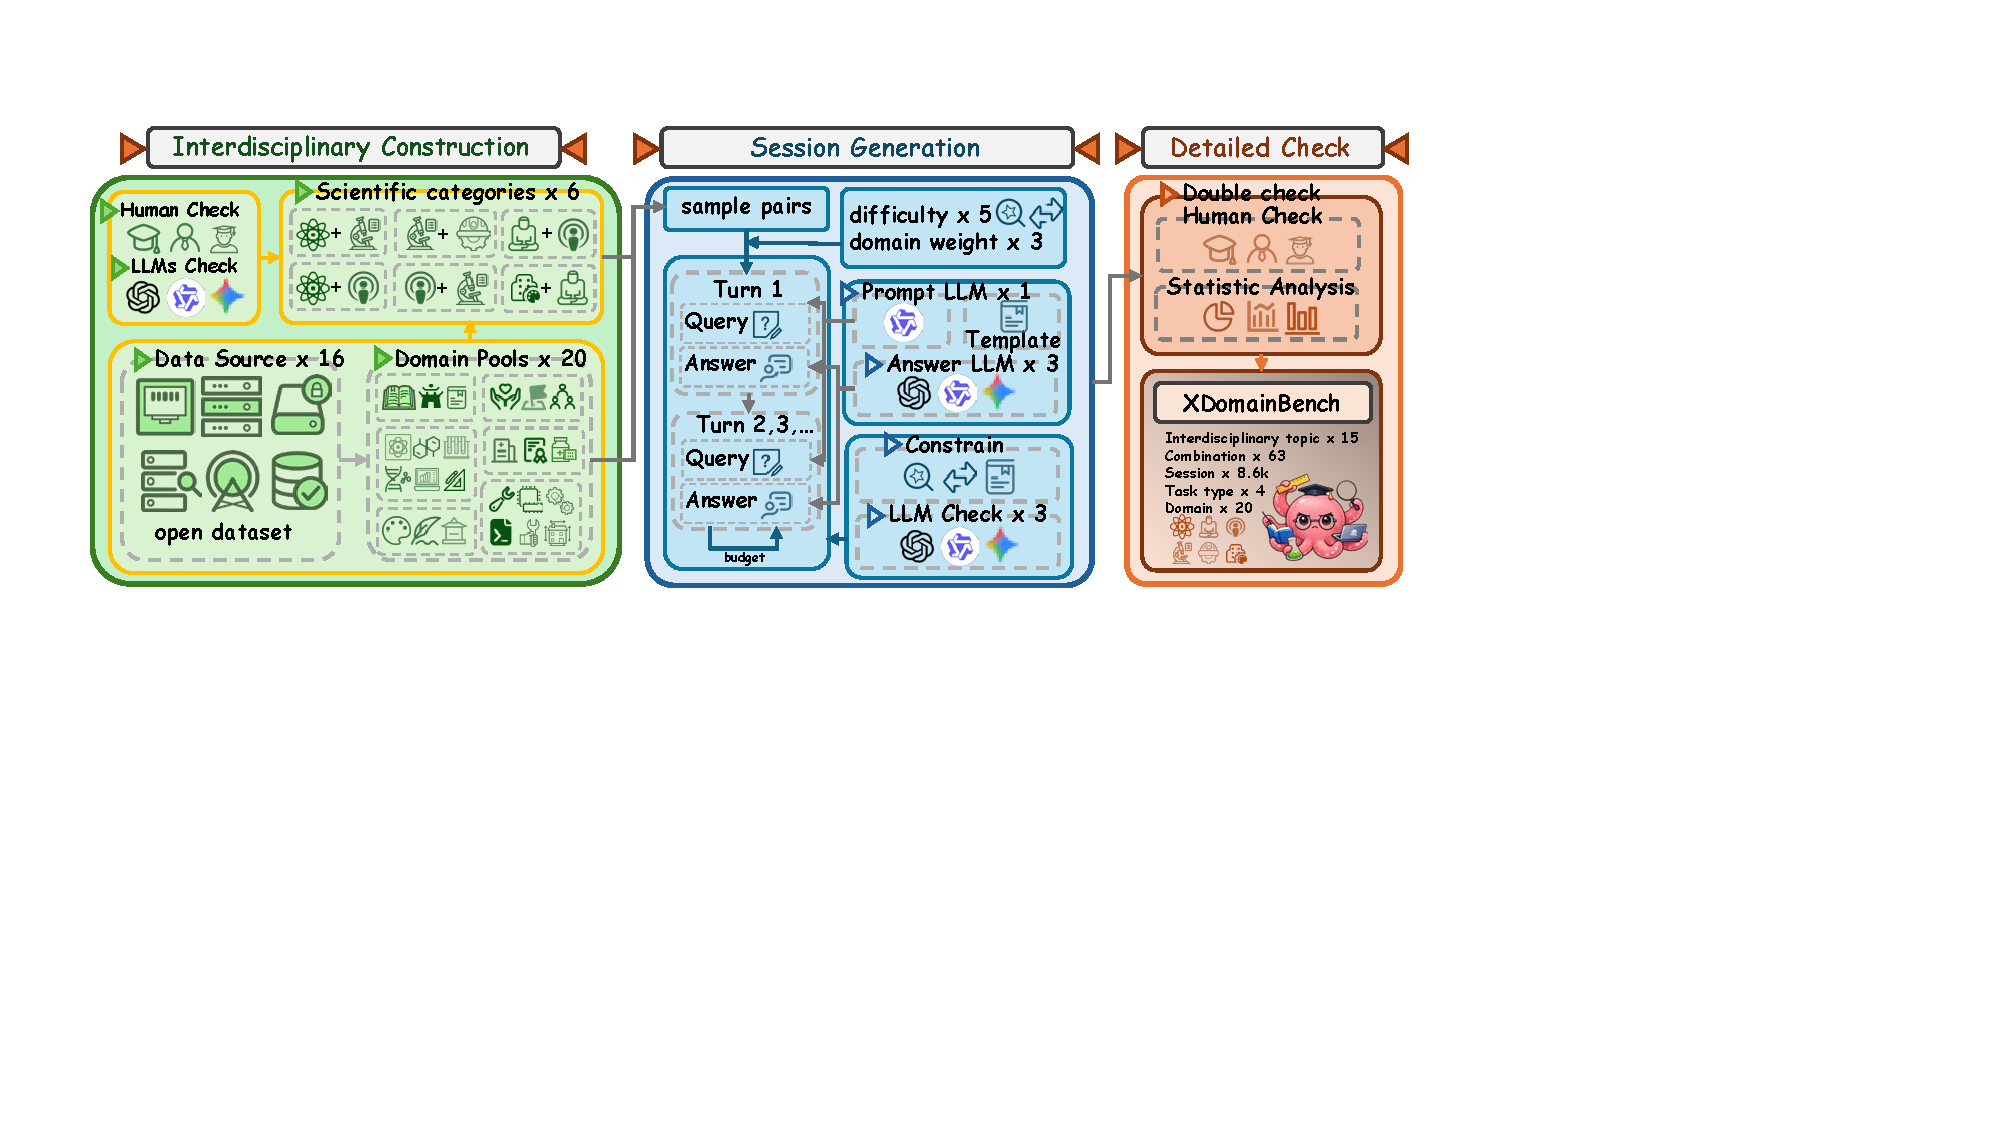
\includegraphics[width=0.98\linewidth]{figures/bench_design.pdf}
    \vspace{-1mm}
    \caption{\textbf{Design framework of \textsc{XDomainBench}} constructing datasets by controlling composition order and mixture structure, generates interactive multi-turn sessions with trajectory-level diagnostic annotations with detailed human check.}
    \vspace{-1mm}
    \label{fig:bench_design}
\end{figure*}

\begin{figure}[!t]
    \centering
    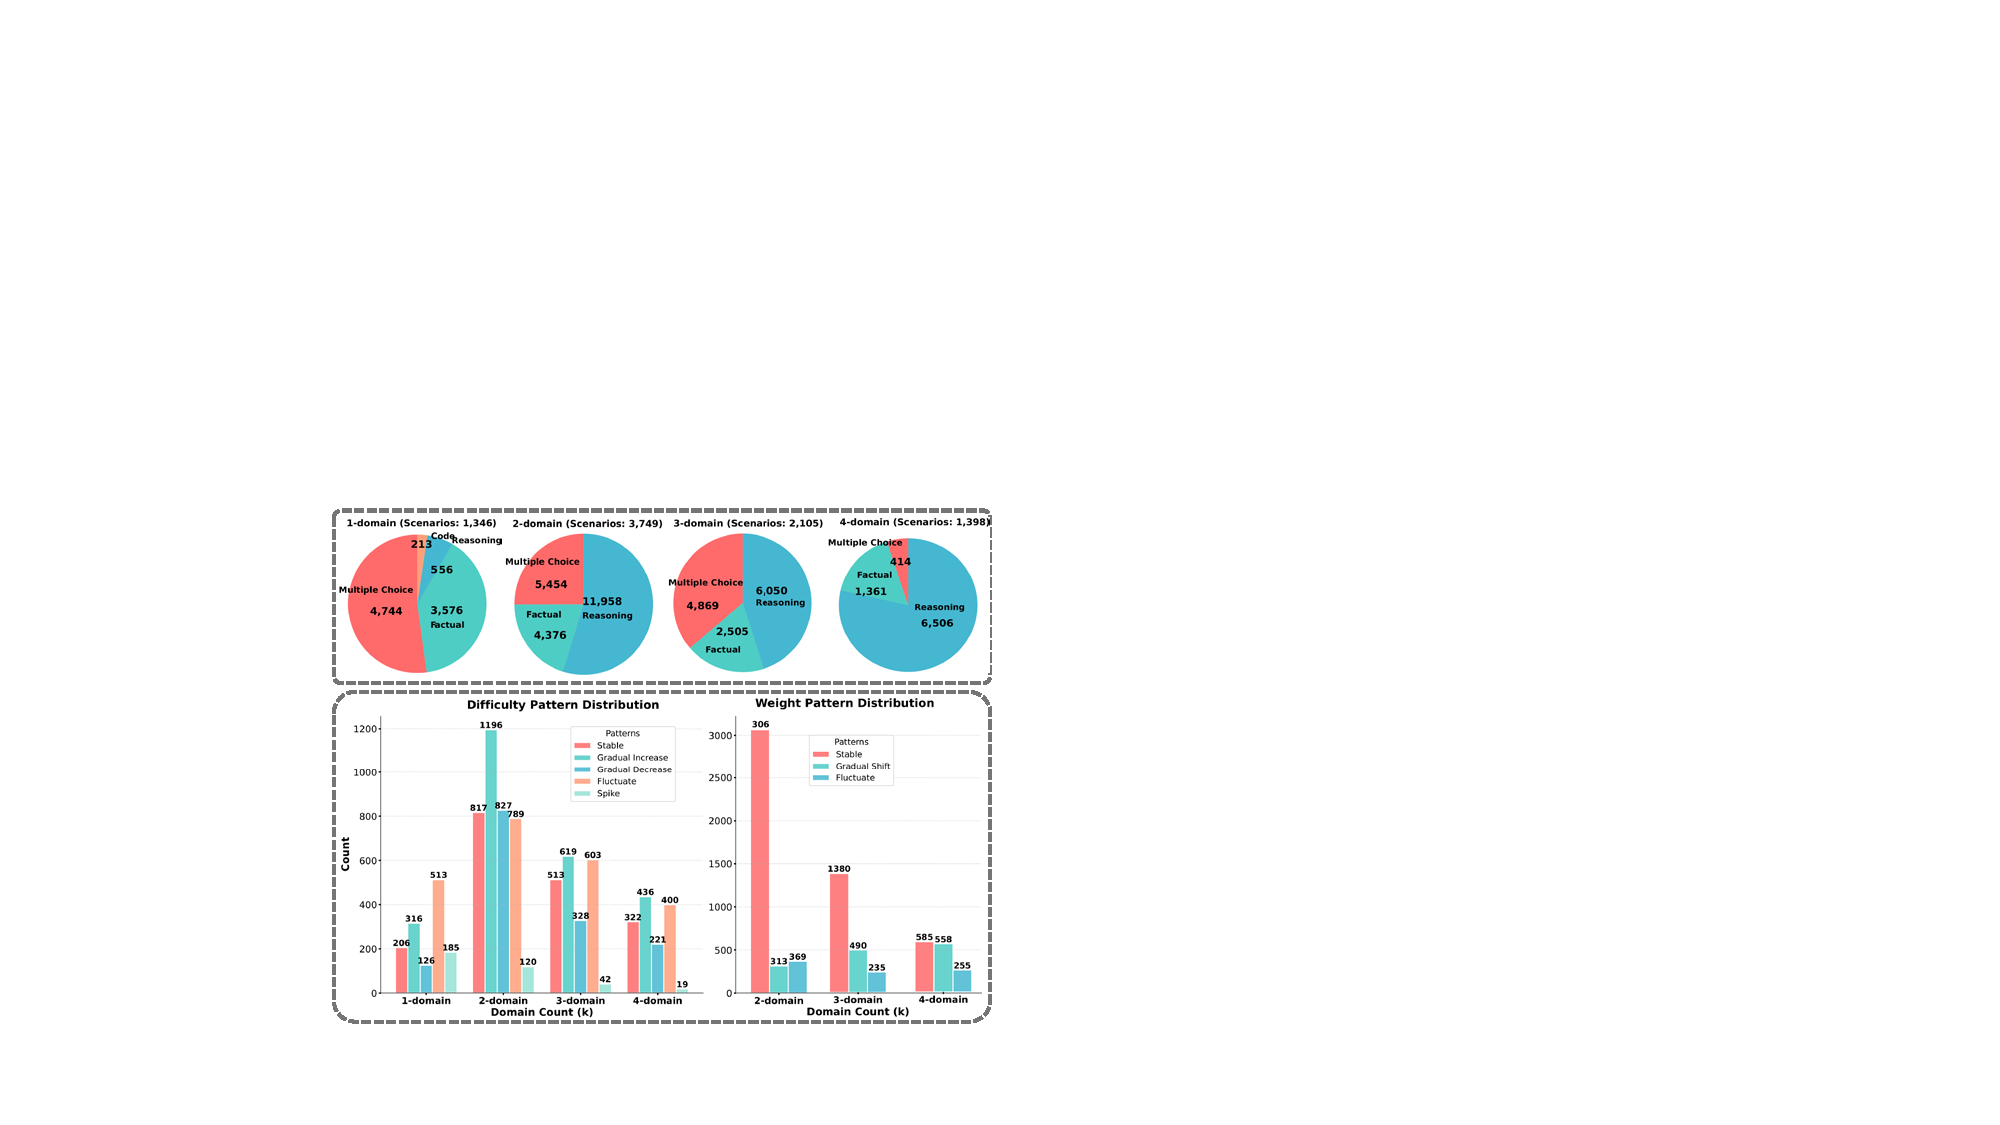
\includegraphics[width=0.98\linewidth]{figures/distribution.pdf}
     \vspace{-2mm}
    \caption{\textbf{Distribution of different patterns and task tpyes} showing content complexity and diagnosability of \textsc{XDomainBench}}
    \label{fig:distribution}
\end{figure}
% ==========================================================
\subsection{Content complexity richness}
\label{sec:complexity_patterns}

We construct sessions with controlled difficulty and domain-mixture trajectories, where conversations evolve through extension, expansion, and deepening around an interdisciplinary topic, simulating realistic AI4S assistance. The distribution is shown in Figure \ref{fig:distribution}. Detailed definitions and thresholds are in Appendix~\ref{app:pattern_taxonomy}. We also validate the reliability $\delta_t$ through detailed human checks and statistical analysis in Appendix~\ref{app:trajectory_annotation}.

\subsubsection{Difficulty trajectory and patterns}
\label{sec:difficulty}

Each session is annotated with per-turn \emph{difficulty scores} $\delta_t \in [0,1]$ to capture how the session's difficulty pattern evolves.
We estimate $\delta_t$ using a hybrid approach: (i) performance-based signals from 3 fixed pilot models to avoid model bias and (ii) semantic complexity proxies.

Each session is assigned one of five difficulty patterns: \textsc{Stable}, \textsc{Gradual Increase}, \textsc{Gradual Decrease}, \textsc{Spike}, and \textsc{Fluctuate}.
Pattern assignment uses interpretable statistics (mean level $\mu_\delta$, volatility $\sigma_\delta$, and trend scores).

\subsubsection{Domain-mixture trajectory and patterns}
\label{sec:mixture}

At each turn $t$, we specify a \emph{domain-mixture distribution} $w_t \in \Delta^{k-1}$ over the selected domains, which governs how strongly the turn should rely on each domain.
We quantify per-turn mixture dispersion using Shannon entropy: $H(w_t) = -\sum_{i=1}^{k} w_{t,i} \log w_{t,i}$.
We measure drift between consecutive turns using Jensen--Shannon divergence: $d_t = \text{JSD}(w_t \,\|\, w_{t+1})$ for $t=2,\ldots,T$.

Each session is annotated with one of three mixture patterns with the trajectory $w_{1:T}$: \textsc{Stable} ($w_t \equiv w_0$), \textsc{Gradual Shift} (interpolation between endpoint mixtures), and \textsc{Fluctuate} (bounded random walk on the simplex).


\subsubsection{Task types}
\label{sec:task_types}

Sessions incorporate four task types to reflect diverse query forms in real AI4S scenarios: \textbf{Multiple Choice} (selection from options), \textbf{Factual QA} (direct knowledge recall), \textbf{Reasoning} (step-by-step derivation), and \textbf{Code} (programmatic solutions).
\footnote{The selection of task types is random and depends on the range of task types available for this cross-disciplinary topic. And to prevent bias in model performance evaluation caused by different distributions of task types, we normalize task types in all subsequent average performance evaluations.}
Each task type has a template family and domain-specific seed pools.


% Define colors for table rows (matching slm_agent paper style)
\definecolor{icmlblue}{RGB}{235, 243, 255}
\definecolor{lightgray}{gray}{0.96}
\definecolor{darkblue}{RGB}{0, 0, 139}

\begin{table*}[!t]
\small
\centering
\caption{\textbf{Overall scaling results as composition order increases ($k=1\rightarrow4$).}
\textbf{Left:} Deterministic problems (R: Recall; F1: F1-score; S@t: SessionSuccess@$\tau$).
\textbf{Right:} Open-world problems. 
To prevent bias caused by task type, the data has been normalized.}
\vspace{-1mm}
\setlength{\tabcolsep}{0.75pt}
\renewcommand{\arraystretch}{1.08}
\begin{adjustbox}{max width=\textwidth}
\begin{tabular}{lccc|ccc|ccc|ccc||ccc|ccc|ccc|ccc}
\toprule
 &  \multicolumn{12}{c}{\textbf{Deterministic Problems}}  &  \multicolumn{12}{c}{\textbf{Open-world Problems}} \\
\cmidrule(lr){2-13} \cmidrule(lr){14-25}
& \multicolumn{3}{c}{\textbf{$k=1$}} & \multicolumn{3}{c}{\textbf{$k=2$}} & \multicolumn{3}{c}{\textbf{$k=3$}} & \multicolumn{3}{c}{\textbf{$k=4$}}
& \multicolumn{3}{c}{\textbf{$k=1$}} & \multicolumn{3}{c}{\textbf{$k=2$}} & \multicolumn{3}{c}{\textbf{$k=3$}} & \multicolumn{3}{c}{\textbf{$k=4$}} \\
\cmidrule(lr){2-4} \cmidrule(lr){5-7} \cmidrule(lr){8-10} \cmidrule(lr){11-13} 
\cmidrule(lr){14-16} \cmidrule(lr){17-19} \cmidrule(lr){20-22} \cmidrule(lr){23-25}
\textbf{Model} & R & F1 & S@t & R & F1 & S@t & R & F1 & S@t & R & F1 & S@t
& R & F1 & S@t & R & F1 & S@t & R & F1 & S@t & R & F1 & S@t \\
\midrule
\rowcolor{lightgray} \multicolumn{25}{c}{\rule{0pt}{1.8ex}\textbf{Large Models}\rule[-0.6ex]{0pt}{0pt}} \\
GPT-5.2              & 30.8 & 22.0 & 42.5 & 25.9 & 11.4 & 28.8 & 22.8 & 8.2 & 25.2 & 18.0 & 4.8 & 26.9 & 25.9 & 9.3 & 29.6 & 21.7 & 7.0 & 28.2 & 28.0 & 5.8 & 21.4 & 13.0 & 5.8 & 35.3 \\
Claude-4.5 Sonnet   & 30.4 & 22.8 & 48.5 & 28.6 & 14.0 & 31.3 & 21.0 & 7.3 & 26.7 & 19.3 & 4.5 & 24.4 & 30.2 & 8.0 & 40.7 & 23.4 & 10.3 & 21.4 & 13.5 & 5.5 & 21.4 & 13.3 & 4.0 & 14.7 \\
Claude-4.5 Haiku    & 30.6 & 23.0 & 41.8 & 29.7 & 13.7 & 31.1 & 26.9 & 12.3 & \textcolor{darkblue}{30.7} & 23.0 & 9.5 & \textcolor{darkblue}{37.7} & 19.4 & 7.0 & 40.7 & 22.4 & 11.0 & 21.4 & 32.6 & 13.8 & 23.2 & 19.1 & 11.5 & 35.3 \\
Gemini-2.5 Flash    & 27.1 & 20.4 & 36.6 & 21.4 & 5.3 & 24.3 & 18.4 & 3.0 & 25.2 & 13.8 & 3.1 & 21.3 & 18.8 & 6.9 & 33.3 & 22.1 & 4.1 & \textcolor{darkblue}{34.2} & 13.5 & 3.3 & 21.4 & 12.4 & 3.7 & 34.5 \\
Gemini-2.0 Flash    & 27.2 & 12.9 & 26.9 & 22.4 & 5.6 & 25.8 & 20.7 & 5.0 & 24.3 & 15.0 & 2.8 & 20.3 & 26.8 & 1.8 & 22.2 & 16.2 & 2.8 & 24.8 & 12.6 & 4.6 & 16.1 & 11.9 & 2.3 & 15.4 \\
Qwen2.5-72B         & 26.8 & 17.8 & 35.8 & 27.0 & 12.8 & 27.3 & 25.0 & 11.5 & 28.2 & 19.9 & 8.9 & 32.3 & 31.3 & 8.4 & 25.9 & 21.9 & 11.2 & 20.5 & 16.1 & 10.2 & 21.4 & 13.2 & 10.3 & 32.4 \\
\rowcolor{icmlblue} \textbf{Mean} & 28.8 & 19.8 & 38.7 & 25.8 & 10.5 & \textbf{28.1} & 22.5 & 7.9 & \textbf{26.7} & 18.2 & 5.6 & 27.1 & 25.4 & 6.9 & 32.1 & 21.3 & 7.7 & \textbf{25.1} & 19.4 & 7.2 & \textbf{20.8} & 13.8 & 6.3 & 27.9 \\
\midrule
\rowcolor{lightgray} \multicolumn{25}{c}{\rule{0pt}{1.8ex}\textbf{Small Models}\rule[-0.6ex]{0pt}{0pt}} \\
GPT-5-mini          & 23.1 & 12.8 & 25.2 & 25.3 & 14.4 & 21.3 & 22.4 & 2.2 & 20.0 & 11.4 & 1.3 & 20.0 & 22.0 & 2.8 & 10.0 & 23.1 & 3.4 & 20.0 & 3.2 & 3.3 & 10.0 & 3.2 & 3.3 & 10.0 \\
Qwen2.5-14B         & 27.2 & 19.1 & \textcolor{darkblue}{39.6} & 25.5 & 11.3 & 26.6 & 23.3 & 9.1 & 27.7 & 18.5 & 7.6 & 29.9 & 18.2 & 3.9 & 18.5 & 27.1 & 10.4 & 25.6 & 28.1 & 9.3 & 10.7 & 11.6 & 7.5 & 20.6 \\
Qwen2.5-7B          & 26.4 & 18.4 & 31.3 & 25.8 & 11.5 & 26.8 & 23.3 & 9.8 & 28.7 & 18.9 & 7.3 & 28.1 & 50.2 & 3.7 & 18.5 & 22.6 & 8.6 & 23.9 & 11.1 & 7.6 & 8.9 & 14.5 & 6.8 & 17.6 \\
Llama-3.1-8B        & 26.2 & 18.8 & 35.8 & 24.7 & 11.4 & 23.8 & 23.3 & 9.9 & 28.2 & 16.5 & 8.1 & 25.1 & 15.2 & 4.1 & 14.8 & 23.9 & 9.8 & \textcolor{darkblue}{29.9} & 28.9 & 10.3 & 17.9 & 19.0 & 7.9 & 29.4 \\
Llama-3.2-3B        & 26.8 & 16.3 & 31.3 & 24.5 & 10.5 & 23.8 & 23.2 & 8.7 & 28.7 & 20.9 & 5.5 & 29.9 & 19.6 & 3.4 & \textcolor{darkblue}{25.9} & 22.8 & 8.9 & 25.6 & 47.1 & 6.9 & \textcolor{darkblue}{23.2} & 14.3 & 5.1 & 26.5 \\
Gemma-2-2B-IT       & 27.3 & 18.6 & 30.6 & 26.3 & 12.1 & 27.6 & 20.6 & 7.4 & 21.8 & 18.1 & 4.3 & 22.6 & 18.4 & 4.6 & 7.4 & 20.7 & 8.5 & 18.8 & 45.0 & 7.4 & 17.9 & 9.5 & 2.8 & 17.6 \\
\rowcolor{icmlblue} \textbf{Mean} & 26.2 & 17.3 & \underline{32.3} & 25.3 & 11.9 & \underline{\textbf{25.0}} & 22.7 & 7.9 & \underline{25.9} & 17.4 & 5.7 & \underline{25.9} & 23.9 & 3.8 & \underline{15.9} & 23.4 & 8.3 & \underline{24.0} & 27.2 & 7.5 & \underline{\textbf{14.8}} & 12.0 & 5.6 & \underline{20.3} \\
\midrule
\rowcolor{lightgray} \multicolumn{25}{c}{\rule{0pt}{1.8ex}\textbf{MoE Models}\rule[-0.6ex]{0pt}{0pt}} \\
Qwen3-Next-80B  & 63.8 & 65.7 & \textcolor{darkblue}{89.6} & 46.3 & 40.1 & \textcolor{darkblue}{51.1} & 41.7 & 36.4 & \textcolor{darkblue}{52.0} & 29.5 & 26.3 & \textcolor{darkblue}{34.5} & 10.8 & 15.0 & \textcolor{darkblue}{40.7} & 29.8 & 27.9 & \textcolor{darkblue}{28.2} & 26.3 & 23.9 & \textcolor{darkblue}{46.4} & 25.7 & 24.1 & \textcolor{darkblue}{41.2} \\
Mixtral-8x7B        & 56.4 & 22.4 & \textcolor{darkblue}{74.6} & 51.9 & 18.0 & \textcolor{darkblue}{46.4} & 51.0 & 18.9 & \textcolor{darkblue}{48.5} & 41.0 & 19.5 & \textcolor{darkblue}{49.4} & 24.1 & 21.3 & \textcolor{darkblue}{40.7} & 41.9 & 25.7 & \textcolor{darkblue}{35.9} & 42.0 & 25.5 & \textcolor{darkblue}{53.6} & 39.9 & 23.7 & \textcolor{darkblue}{55.9} \\
\rowcolor{icmlblue} \textbf{Mean} & 60.1 & 44.0 & \underline{82.1} & 49.1 & 29.1 & \underline{\textbf{48.8}} & 46.4 & 27.6 & \underline{50.2} & 35.2 & 22.9 & \underline{\textbf{42.0}} & 17.5 & 18.1 & \underline{40.7} & 35.9 & 26.8 & \underline{\textbf{32.0}} & 34.1 & 24.7 & \underline{50.0} & 32.8 & 23.9 & \underline{\textbf{48.5}} \\
\bottomrule
\end{tabular}
\end{adjustbox}
%\vspace{-1mm}
\label{tab:overall_scaling}
\end{table*}
% ==========================================================
\subsection{Diagnosability}
\label{sec:diagnostic_signals}

We attribute performance degradation to two root causes: (i) \emph{direct}: insufficient capability for handling complex high-dimensional scientific knowledge composition; (ii) \emph{indirect}: performance degradation induced by session pattern dynamics in multi-turn interactive scenarios.

\subsubsection{Direct mechanism: Turn-level compositional difficulty}
\label{sec:direct_mechanism}

The direct mechanism manifests as immediate difficulty increases when domain combinations increase, as higher-dimensional compositions raise cognitive load and joint reasoning ability.
We diagnose this using the difficulty trajectory $\{\delta_t\}_{t=1}$ with its relationship to composition order $k$, since the initial step questions are directly sampled from single-domain pools during our session construction.

\subsubsection{Indirect mechanism: Session-level interactive dynamics}
\label{sec:indirect_mechanism}

The indirect mechanism operates through difficulty and domain-mixture dynamics in multi-turn interactive sessions.
We formalize this via three interaction-level failure phenomena to mediate how trajectories with different patterns lead to session-level degradation:
\textbf{Error accumulation} (sustained performance decline after an onset turn), \textbf{Reasoning breaks} (sudden accuracy drops indicating model failure to maintain reasoning continuity), and \textbf{Domain confusion} (realized domain reliance deviates from intended mixture).
Each phenomenon is detected via reproducible heuristics combining standardized signals (Judge scores $J_t$, ParseFail indicators $\text{PF}_t$, mixture mismatches $d_t$) with judge-assisted verification when needed.
Operational definitions, detector rules, and signature curves are detailed in Appendix~\ref{app:pattern_taxonomy}.

\begin{figure}[!t]
  \centering
  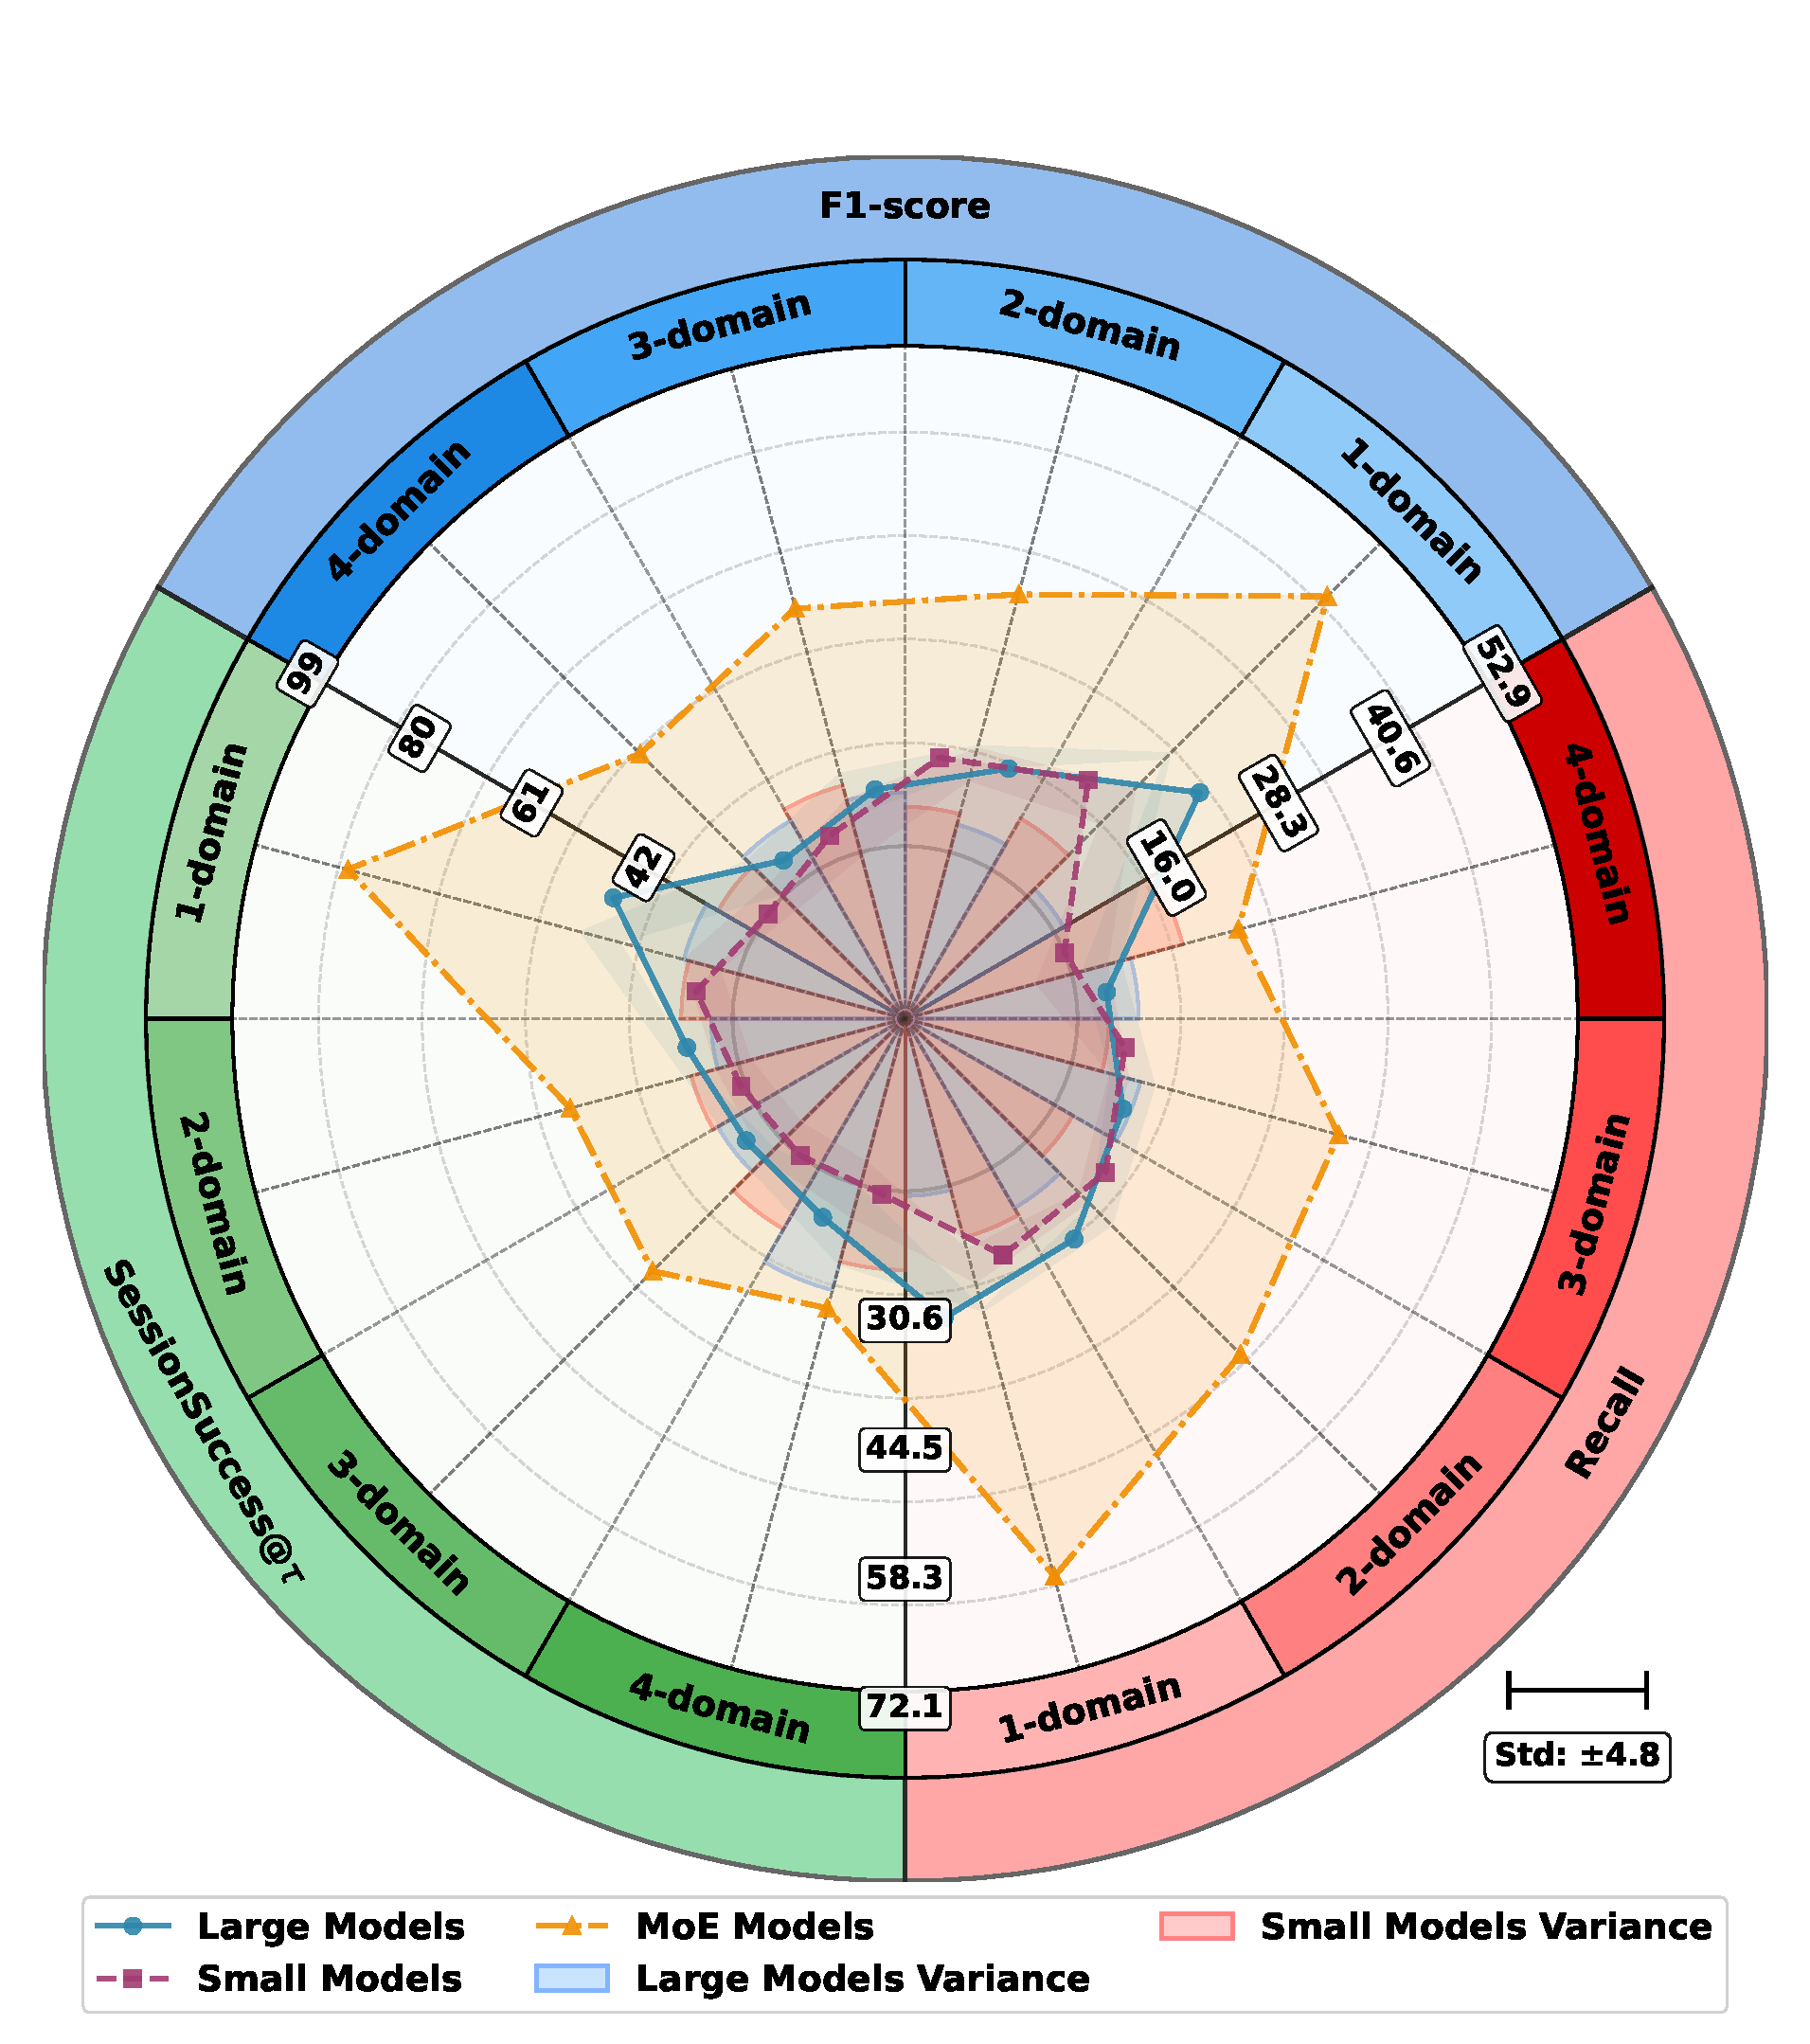
\includegraphics[width=\linewidth]{figures/radar_scaling.pdf}
  \caption{\textbf{Multi-metric scaling patterns across composition orders.}
   Variance bands illustrate that small models exhibit greater sensitivity to composition order.}
%   \vspace{-1mm}
  \label{fig:radar_scaling}
\end{figure}

\begin{figure*}[!t]
  \centering
  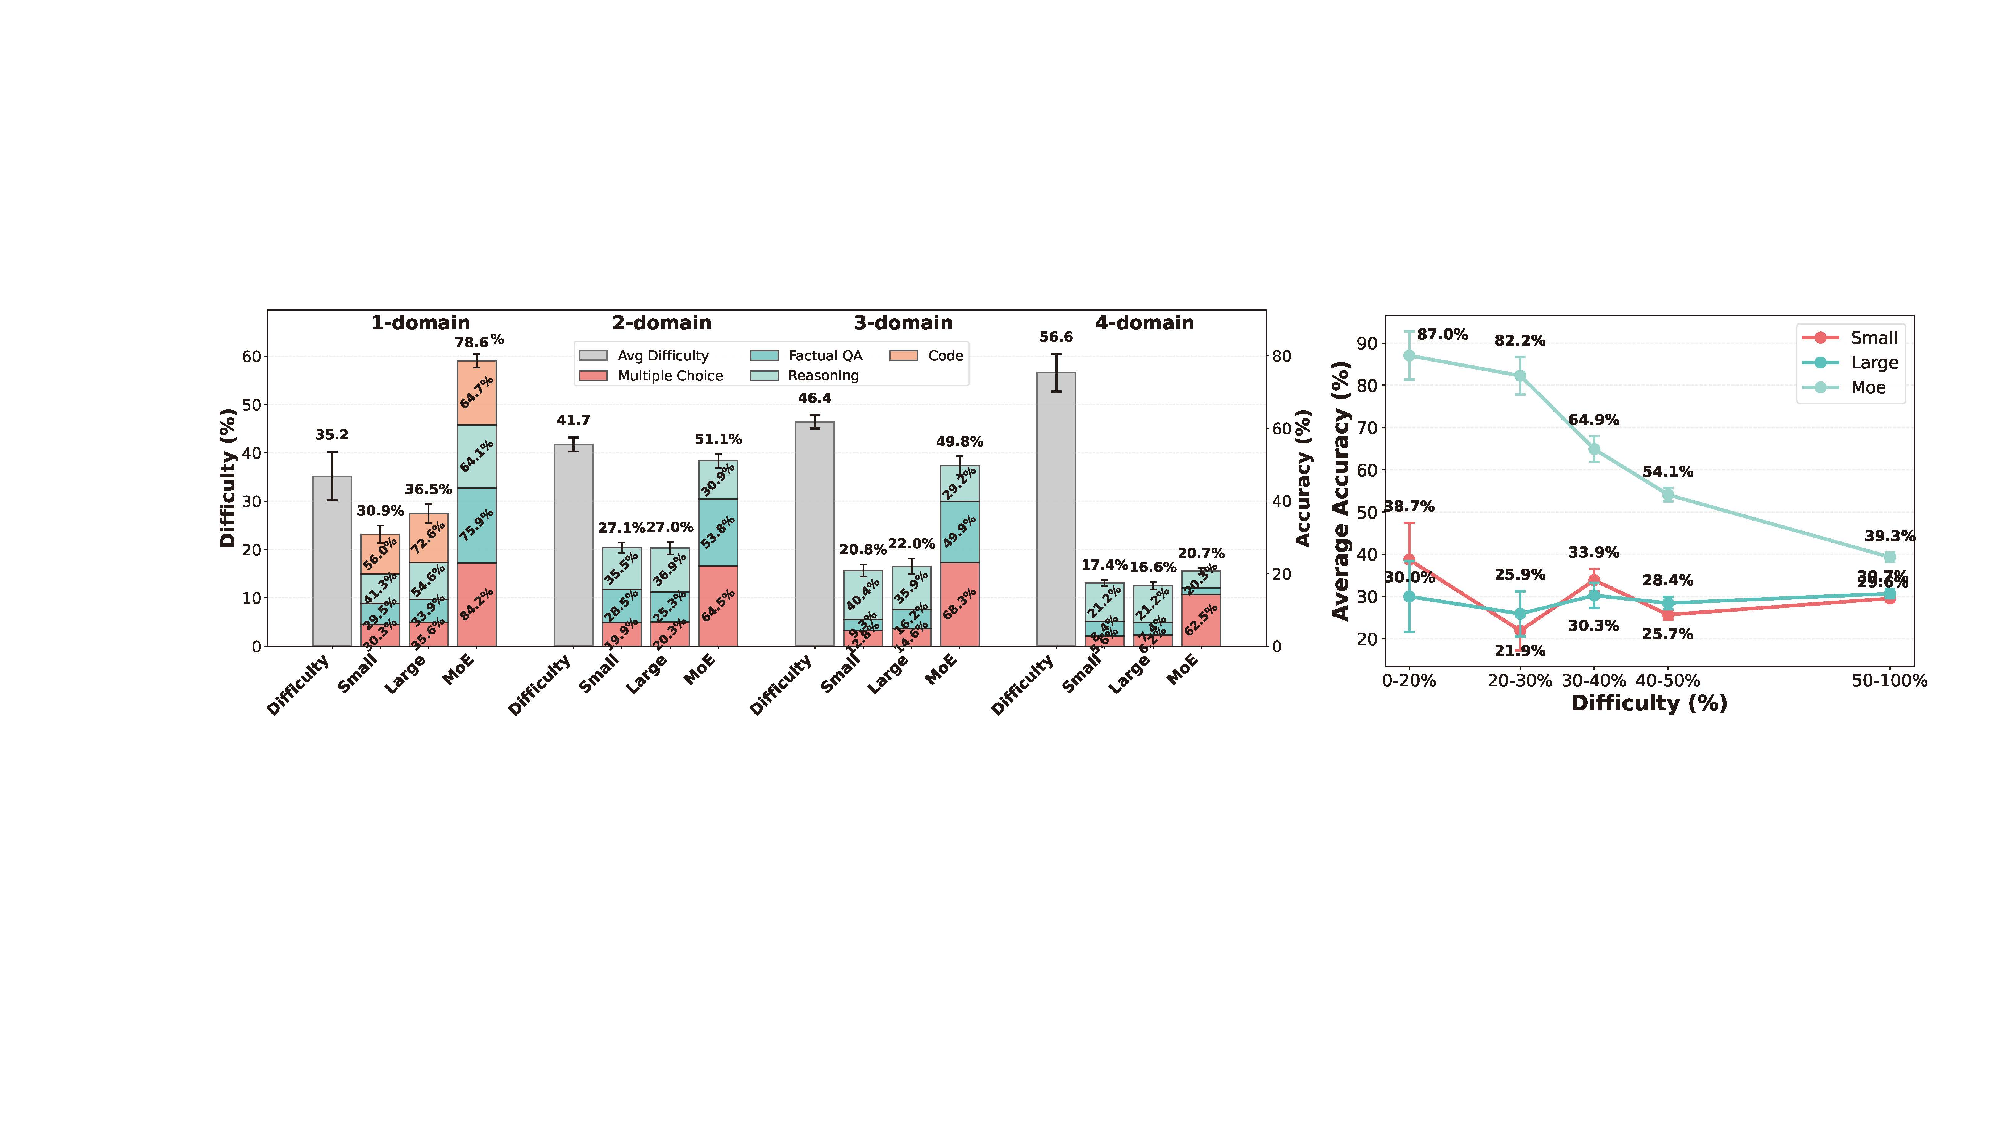
\includegraphics[width=0.99\linewidth]{figures/turn1_barplot1.pdf}
  \vspace{-1mm}
  \caption{Left: \textbf{Performance breakdown by composition order and task type at Turn 1.}
  Each group contains average difficulty and performance for small, large, and MoE models. Right: \textbf{Performance vs. difficulty by model type.}}
  \label{fig:turn1_barplot}
\end{figure*}
% ==========================================================
\subsection{Dataset construction pipeline}
\label{sec:episode_construction}

Following the construction pipeline shown in \cref{fig:bench_design},
we summarize the three-stage process:

\textbf{Stage 1: Interdisciplinary construction.}
We first select a domain set $\mathcal{D} = \{d_1, \ldots, d_k\}$ using embedding-based nearest-neighbor policy (Sec.~\ref{sec:composition_space}).
We also use LLM to determine whether the selected domains can form a realistic interdisciplinary scenario, followed by human sanity checks.

\textbf{Stage 2: Session generation.}
For each session with a fixed topic, we first formalize a target configuration $\mathsf{cfg} = (k, P^\delta, P^w)$, where $P^\delta$ and $P^w$ are pattern labels related to difficulty and domain mixture (\cref{sec:complexity_patterns}).
We then instantiate target diagnostic signals: (i) difficulty trajectory $\{\delta_t\}_{t=1}^{T}$ with pattern $P^\delta$ and (ii) mixture trajectory $\{w_t^{\text{target}}\}_{t=1}^{T}$ with regime $P^w$.
For turn 1, an LLM generates a cross-domain question $(x_1, y_1)$ conditioned on $(\mathcal{D}, \delta_1, w_1^{\text{target}})$ and construction templates.
Three state-of-the-art models independently assess the realized domain weight $\hat{w}_1^{\text{realized}}$ and difficulty $\hat{\delta}_1$.
For subsequent turns ($t \geq 2$), generation is conditioned on the previous 1--2 turns to ensure topic coherence, with each turn validated by the same three-model ensemble.
If validation fails (e.g., $\hat{w}_t^{\text{realized}}$ deviates from $w_t^{\text{target}}$ beyond tolerance), the turn is regenerated until constraints are met or a retry budget is exhausted.
To ensure accuracy, three models provide answers for each turn, while identical answers are merged and samples with large differences in model responses will be deleted.

\textbf{Stage 3: Detailed check.}
After all turns are generated, we verify that the realized session matches the intended difficulty pattern $P^\delta$ and mixture regime $P^w$.
If constraints are violated, we resample affected turns or resample targets, then rerun validation under a bounded session retry budget.
Finally, all accepted sessions undergo detailed human quality checks and expert review for critical cases.
\vspace{-0.5mm}

\paragraph{Decoupling construction and evaluation.}
Construction-time LLMs are used only to instantiate, validate, and calibrate candidate sessions under fixed diagnostic targets.
They do not define the evaluation target and are not used to score the tested models in the default protocol.
The evaluated quantity is the model's degradation pattern under controlled composition orders and trajectory regimes, 
not agreement with the construction models.
This separation reduces the risk that benchmark performance merely reflects generator imitation.
\vspace{-0.5mm}

\paragraph{Role of public seed pools.}
Public QA sources are used only as seed pools for anchoring feasible domain concepts and supervision formats.
They are not directly reused as the evaluated multi-turn sessions.
Each released session is newly instantiated through controlled generation and validation, where later turns vary in topic realization, task form, difficulty, and domain-mixture trajectory while remaining coherent under the same interdisciplinary scenario.
Thus, \textsc{XDomainBench} evaluates newly constructed interactive sessions rather than recycled public benchmark items.
\vspace{-0.5mm}

%\paragraph{Quality assurance.}
%We curate reference answers using a hybrid approach: LLM-assisted generation, expert review for critical cases, and cross-annotation agreement checks~\citep{li2024arenahard,zhou2023instruction}.
%We implement safeguards against benchmark leakage and contamination~\citep{deng-etal-2024-investigating}.
%Detailed curation policies, filtering rules, and audit examples are in Appendices~\ref{app:dataset_construction} and \ref{app:data_quality}.
